

The following describes the classes and subclasses used to create the ontology in Protege.
\\

\begin{itemize}
    \item \textbf{Classes} (that are subclasses of owl:Thing):
    \begin{itemize}
        \item Organism;

        \item Habitat;

        \item Resource.
        \\
    \end{itemize}

    \item \textbf{Subclasses}:
    \begin{itemize}
        \item Animal, Plant and Microorganism as subclasses of Organism (all mutually disjoint from each other);

        \item Herbivore, Carnivore and Omnivorous as subclasses of Animals, where Omnivorous is defined as Herbivore $\cap$ Carnivore;

        \item Bryophytes and  Angiosperms as subclasses of Plants (all mutually disjoint from each other).
        \\
    \end{itemize} 
\end{itemize}

It is important to note that all classes and subclasses are mutually exclusive; therefore, no individual from one class can belong to another, and no individual from one subclass can belong to another subclass. The hierarchy of classes can be better observed in the figure below.

\begin{figure}[H]
    \centering
    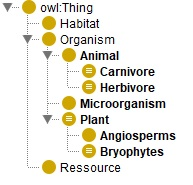
\includegraphics[width=0.35\linewidth]{images/ontology/classes.jpg}
    \caption{Class hierarchy}
    \label{fig:class}
\end{figure}


Regarding the Class properties, we have the following \textbf{Data properties}:
\\

    \begin{itemize}
        \item \textit{weight} with domain Animal and range xsd:decimal;

        \item \textit{has\_Fruits} with domain Plant and range xsd:boolean. In addition, this property is set to be True for Angiosperms and False for Briophites;

        \item \textit{chemical\_formula} with domain Ressource and range xsd:string;

        \item \textit{scientific\_name} with domain Organism and range xsd:string.
        \\

    \end{itemize}


The following two figures illustrate both the declaration of data properties and the method used to ensure the uniqueness of the \textit{scientific\_name}, for example.
\\

\begin{figure}[H]
    \centering
    \begin{minipage}{0.35\textwidth}
        \centering
        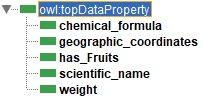
\includegraphics[width=\textwidth]{images/ontology/mini1.jpg}
        \caption{Data properties}
        \label{fig:figura1}
    \end{minipage}%
    \hspace{0.1\textwidth}
    \begin{minipage}{0.35\textwidth}
        \centering
        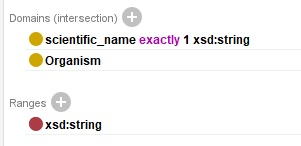
\includegraphics[width=\textwidth]{images/ontology/mini2.jpg}
        \caption{Unique property}
        \label{fig:figura2}
    \end{minipage}
\end{figure}

Finally, we have the following \textbf{Object properties}:
\\

    \begin{itemize}
        \item \textit{eat} with domain Animal and range Organism. This property is also irreflexive;

        \item \textit{foundInHabitat} with domain Organism and range Habitat;

        \item \textit{consumeTheResource} with domain Organism and range Resource;

        \item \textit{isEatenBy} with domain Organism and range Animal (is the inverse property \textit{eat});

        \item \textit{isNotEatenBy} with domain Animal $\cup$ Plant and range Animal. It's disjoint with \textit{isEatenBy};

        \item \textit{isOccupiedBy} with domain Habitat and range Organism (is the inverse of \textit{foundInHabitat});

        \item \textit{hasTheResource} with domain Habitat and range Resource;

        \item textit{isConsumedBy} with domain Resource and range Organism (is the inverse of \textit{consumeTheResource});

        \item \textit{isInTheHabitat} with domain Resource and range Habitat (inverse of the property \textit{hasTheResource})

        \item \textit{coExistWith} with domain Organism and range Organism. This property is symmetric. In addition, this property is different if both organisms are animals/plants or if they are both microorganisms:
        \begin{enumerate}
            \item $A$ and $B$ are herbivores/plants: \textit{A} coexists with \textit{B} means that \textit{A} and \textit{B} lives at the same environment (foundInHabitat(A) == foundInHabitat(B));

            \item $A$ and $B$ are both microorganisms: \textit{A} coexists with \textit{B} means that \textit{A} and \textit{B} lives at the same environment (foundInHabitat(A) == foundInHabitat(B)) \textbf{and} they do not consume the same resource through the relation consumeTheResource;

            \item $A$ and $B$ are carnivores: \textit{A} coexists with \textit{B} means that \textit{A} and \textit{B} lives at the same environment (foundInHabitat(A) == foundInHabitat(B)) \textbf{and} they do not share neither the relation \textit{A isNotEatenBy B} and \textit{B isNotEatenBy A};
            \\
            
        \end{enumerate}
    \end{itemize}

Finally, if two Organisms coexists, it means that they should be both at the same Habitat:

$$foundInTheHabitat(A, Hab)
\land coExistWith(A, B) \rightarrow
foundInTheHabitat(B, Hab)$$

The list of object properties in Protege can be seen in the figure below.

\begin{figure}[H]
    \centering
    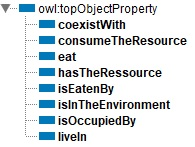
\includegraphics[width=0.35\linewidth]{images/ontology/obg_protp.jpg}
    \caption{Object properties}
    \label{fig:obj}
\end{figure}

The inference rules were described using \textit{SWRL} (Semantic Web Rule Language), which allows for writing it in a practical and concise manner. Below, we provide a detailed description of all the inference rules related to object and data properties.
\\

We start by the following inference rule: if Organism $a$ eat Organism $b$, and Organism $a$ live in the Habit $env$, then $b$ should also live in $env$. This is described by:
\\

\begin{lstlisting}
eat(?a, ?b) ^ foundInHabitat(?a, ?env) -> foundInHabitat(?b, ?env)
\end{lstlisting}

Regarding the consumption of resources, we have the following equivalence: if Organism $A$ consume Resource $R$ and $A$ is in the Habitat $H$, then $R$ can be found in $H$. In addition, if Resource $R$ can be found in the Habitat $H$ and Organism $A$ consumes this resource, then $A$ lives in $H$. This can be described using SWRL by the following 2 statements:
\\

\begin{lstlisting}
consumeTheResource(?a, ?r), foundInTheHabitat(?a, ?h) -> isInTheHabitat(?r, ?h)
\end{lstlisting}

\begin{lstlisting}
consumeTheResource(?a, ?r), isInTheHabitat(?r, ?h) -> foundInTheHabitat(?a, ?h)
\end{lstlisting}


The same way, if Organism $a$ coexists with Organism $b$, and $a$ live in the Habitat $env$, $b$ should also live in $env$.
\\

\begin{lstlisting}
coexistWith(?a, ?b) ^ foundInHabitat(?a, ?env) -> foundInHabitat(?b, ?env)
\end{lstlisting}


From now on, we will focus on discussing the coexistence relationship, which is the most complex relation of the ontology. As previously described, according to our rules, a carnivorous animal will always coexist with another carnivorous animal as long as they inhabit the same environment and they share the relation isNotEatenBy. Additionally, we add the rule that animal $a$ must be different from $b$, as we do not want the relation to be reflexive:


\begin{lstlisting}
Carnivore(?a), Carnivore(?b),  DifferentFrom (?a, ?b), foundInTheHabitat(?a, ?h), foundInTheHabitat(?b, ?h), isNotEatenBy(?a, ?b), isNotEatenBy(?b, ?a) -> coexistWith(?a, ?b)
\end{lstlisting}

We use the same logic to describe the coexistence for the herbivores, as follows:
\\

\begin{lstlisting}
Herbivore(?a), Herbivore(?b),  DifferentFrom (?a, ?b), foundInTheHabitat(?a, ?h), foundInTheHabitat(?b, ?h) -> coexistWith(?a, ?b)
\end{lstlisting}

Next, we have the case of coexistence between plants, which is similar to the herbivore's case:
\\

\begin{lstlisting}
Plant(?a), Plant(?b),  DifferentFrom (?a, ?b), foundInTheHabitat(?a, ?h), foundInTheHabitat(?b, ?h) -> coexistWith(?a, ?b)
\end{lstlisting}

Finally, the coexistence between two microorganism happens when they both live in the same environment \textbf{and} do not consume the same resource: 
\\

\begin{lstlisting}
Microorganism(?a), Microorganism(?b),  DifferentFrom (?a, ?b), foundInTheHabitat(?a, ?h), foundInTheHabitat(?b, ?h), consumeTheResource(?a, ?r), consumeTheResource(?b, ?s),  DifferentFrom (?r, ?s) -> coexistWith(?a, ?b)
\end{lstlisting}